% !TEX root = main.tex

\section{Apple ARKit}
Das ARKit von Apple ist ein Augmented-Reality-Framework, welches mit iOS 11 veröffentlicht wurde \cite{apple_arkit}. ARKit und ARCore sind in ihrem Aufbau sehr ähnlich, sowohl in den Konzepten, als auch in den Schnittstellen. In Tabelle \ref{arkit_vs_arcore} ist dies verdeutlicht.

\begin{table}[h]
	\centering
	\begin{tabular}{|p{4cm}|p{4cm}|}
		\hline
		\textbf{ARKit} & \textbf{ARCore}\\
		\hline
		\multicolumn{2}{|c|}{\textbf{Konzepte}}\\
		\hline
		Visual Inertial Odometry & Motion Tracking\\
		Scene Understanding & Environmental Understanding\\
		Light Estimation & Light Estimation\\
		\hline
		\multicolumn{2}{|c|}{\textbf{Schnittstellen}}\\
		\hline
		ARAnchor & Anchor \\
		ARConfiguration & Config\\
		ARFrame & Frame\\
		ARHitTestResult & HitResult\\
		ARLightEstimate /
		\newline ARDirectionalLightEstimate & LightEstimate\newline\\
		ARPlaneAnchor & Plane\\
		ARSession & Session\\
		ARFaceAnchor & ---\\
		ARCamera & ---\\
		\hline
	\end{tabular}
	\caption{Gegenüberstellung von Apple ARKit\cite{arkit_reference} und Google ARCore\cite{arcore_android_reference}}
	\label{arkit_vs_arcore}
\end{table}

Womit das ARKit hervorsticht ist die "`Face-Based AR Experience"'. Mithilfe der "`TrueDepth Camera"' als Front-Kamera des iPhones kann die Position und das Aussehen des Gesichts erfasst werden und z.B. auf ein virtuelles Gesicht übertragen werden. Ein weiterer Punkt ist das komplette ausblenden des Hintergrunds.\cite{iphoneX}

Die Technologie dahinter ist der Tango-Hardware sehr ähnlich. Es gibt einen Infrarotsensor und einen "`Dot-Projector"', wodurch die Tiefe der Szene, also des Gesichts, ermittelt wird. \cite{iphoneX_display}

Ein beliebtes Genre für AR-Apps ist das Messen der Länge oder Größe von realen Objekten. Dazu gibt es eine Vielzahl von Apps im Apple Appstore, z.B. die aktuell bestbewerteten "`AirMeasure"' oder "`3-in-1 Ruler"'. Google ist diesem Trend zuvorgekommen und liefert mit dem Tango-Gerät eine eigene vorinstallierte App namens "`Measure"' mit. Mit diesen Applikationen lässt sich aber auch gut die Präzision der beiden Plattformen testen. Die Ergebnisse der Messungen sind in Tabelle \ref{ar_measure_apps_comparison} zu sehen.

Google Measure unterscheidet sich um wenige Zentimeter von den realen Maßen. Die Differenzen entstehen zum Großteil aufgrund der Benutzeroberfläche der App. In der Mitte der App befindet sich ein Punkt mit dem die Endpunkte der Strecke markiert werden. Aufgrund der Größe dieses Punktes wird allerdings das präzise Platzieren der Endpunkte erschwert.

Die ARKit Apps sind gerade bei kleineren Strecken ziemlich präzise. Bei eher längeren Strecken wie z.B. der Länge des Türrahmens ist die Abweichung hier jedoch ziemlich groß. Eine der Apps war nicht in der Lage diese Messung durchzuführen. Der Grund hierfür liegt bei ARKit, welches vertikale Flächen nicht wahrnehmen kann. In der Referenz zur ARWorldTrackingConfiguration ist zu erkennen, dass die Plane Detection lediglich auf "`horizontal"' eingestellt werden kann \cite{arkit_reference_config}. Es ist aber wie bei ARCore hier möglich, dass dies demnächst noch hinzugefügt wird.
Lange horizontale Flächen werden mit eine ähnlichen Abweichung wie die restlichen Messwerte gemessen.

Durch die Abwesenheit von vertikalen Flächen wird die Möglichkeit von Verdeckung, also die Verdeckung von virtuellen Objekten durch reale Objekte auch sehr erschwert, da die Verdeckung oft durch vertikale Flächen verursacht wird. Ein Feature, welches in Google Tango vorhanden war.

Des Weiteren ist die Bedienung der Apps etwas schwieriger. Das Gerät benötigt einige Sekunden um die Fläche zu tracken und das zu messende Objekt muss vor der Messung aus mehreren Positionen abgefilmt werden. Letzteres ist ein starkes Indiz dafür, dass beim ARKit Stereoskopie zum Einsatz kommt, d.h. die Tiefe in den Bildern wird aus mehreren Kamerabildern berechnet. Es wird eine zweite Kamera simuliert. Sobald eine horizontale Ebene erfasst wurde und immer solch eine Ebene im Bild war, war das Tracking in den Tests störungsfrei. Ein platziertes Objekt kann in Abbildung \ref{example_app_arkit} gesehen werden. Das Objekt steht dabei direkt auf dem Boden und bleibt bei Bewegungen an der gleichen Stelle. Im Vergleich zu Google Tango ist dies mindestens genauso gut, wenn nicht sogar etwas stabiler.

Beim Probieren mehrerer Apps war keine dabei, die es ermöglicht platzierte Objekte an einer Stelle zu speichern. Aus diesem Grund vermute ich, dass ein Feature wie das Area Learning im ARKit nicht existiert. Auch in den Schnittstellendokumentationen habe ich dazu nichts gefunden. Was es jedoch mehrfach gab, ist dass die virtuellen Objekte gespeichert werden kann, aber beim Laden vom Nutzer neu platziert werden müssen.

\begin{table}[h]
	\centering
	\begin{tabular}{|p{1.9cm}|p{1.74cm}|p{1.74cm}|p{1.74cm}|}
		\hline
		& \textbf{Tisch} & \textbf{Türrahmen} & \textbf{Smartphone}\\
		\hline
		\textbf{Zollstock} & 100x60 & 199x83 & 14,5x7\\
		\hline
		\textbf{Goole Measure} & 98x58 & 200x84 & 13x6\\
		\hline
		\textbf{AirMeasure}& 99,3x58,4 & 190x80,9 & 14,2x7,8\\
		\hline
		\textbf{3-in-1 Ruler} & 98,8x59,3 & XXXx80,5 & 13,7x6,7\\
		\hline
	\end{tabular}
	\caption{Tests von Apps, die reale Objekte abmessen (Maße in cm)}
	\label{ar_measure_apps_comparison}
\end{table}

\begin{figure}[h]
	\centering
	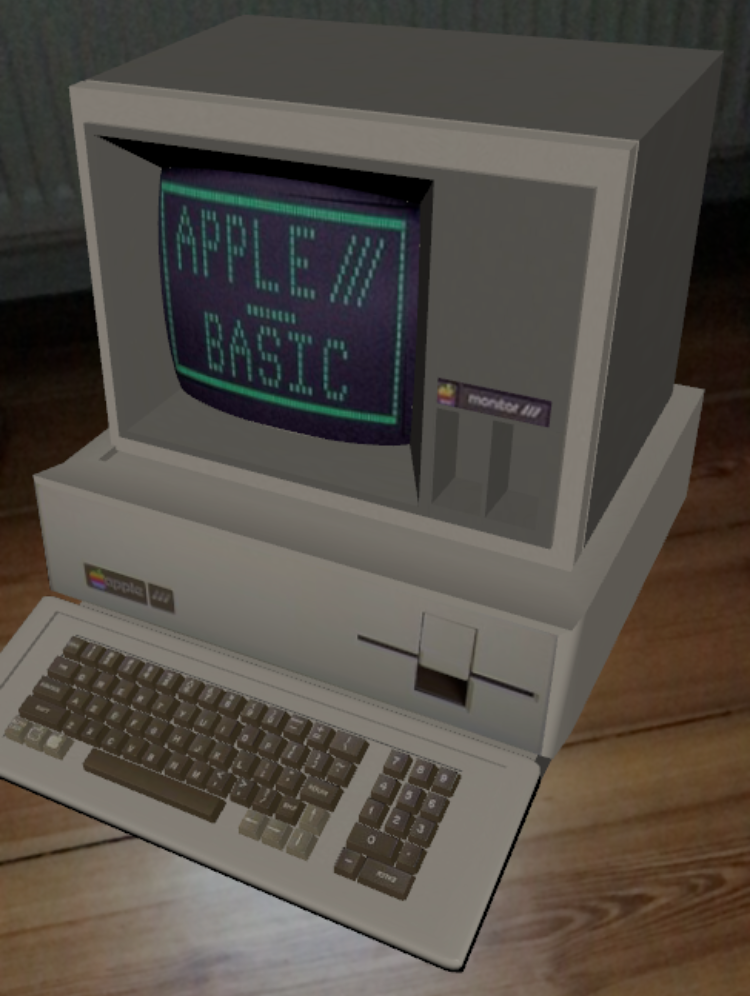
\includegraphics[width=3in]{pictures/arkit_object}
	\caption{Virtuelles Objekt wird in die reale Welt projiziert (ARKit)}
	\label{example_app_arkit}
\end{figure}

